\section{Experiment 2}
\label{sec:exp2}
Experiment 2, similarly to experiment 1, trains and evaluates ANNs for the task to classify images of fruits and vegetables. Experiment 2, however, considers 131 labels, making the classification task more challenging. The goal of the experiment, as in experiment 1, is to try different network types in order to find the best configuration, i.e., the configuration with the lowest Zero-One loss, and to see if the best configuration for experiment 1, still holds for experiment 2.

\subsection{Setup}
The setup is very similar to experiment 1. The experiment is run on the same machine, using networks build by the \texttt{models.py} script.

\textbf{Dataset.} The same dataset of images is used, however all the 90380 images and all the 131 labels are considered this time. For this reason, datasets are managed by a different script, \texttt{dataset\_2.py}, and they are stored in a different folder.

\subsection{Results}
The results collected are summarized in table\ref{table:exp2}.
\input exp2_table

Figure\ref{fig:e2_loss_epochs} shows the zero-one loss and the number of epochs of each ANNs, differentiating the DNNs from the CNNs. The lowest losses are achieved by CNNs, however the chart is very scattered and also many DNNs achieve a very low loss.
\begin{figure}
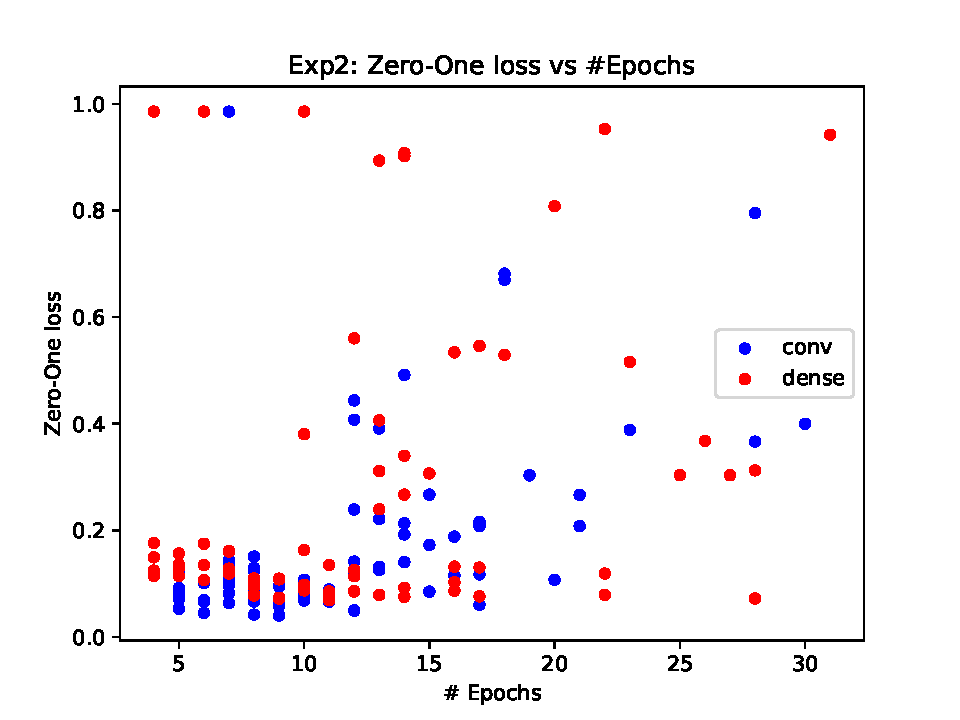
\includegraphics[width=\textwidth]{e2_loss_epochs}
\caption{Experiment 2: zero-one loss vs epochs}\label{fig:e2_loss_epochs}
\end{figure}

Figure\ref{fig:e2_50_loss_width} shows the zero-one loss achieved on images of size 50x50 pixels by ANNs of different depth and width, of type DNN and CNN respectively. The figures show that deeper and wider networks achieve a lower zero-one loss. Note that there is no overfitting in that data because the zero-one loss is computed on the testing set.
\begin{figure}
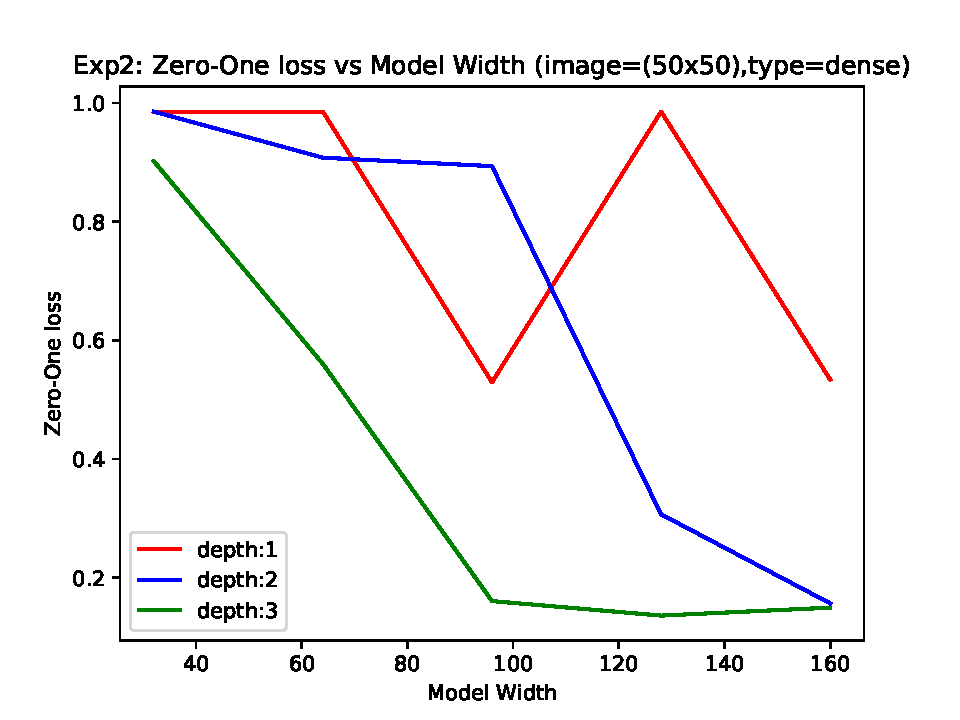
\includegraphics[width=\textwidth]{e2_50_dense_loss_width}
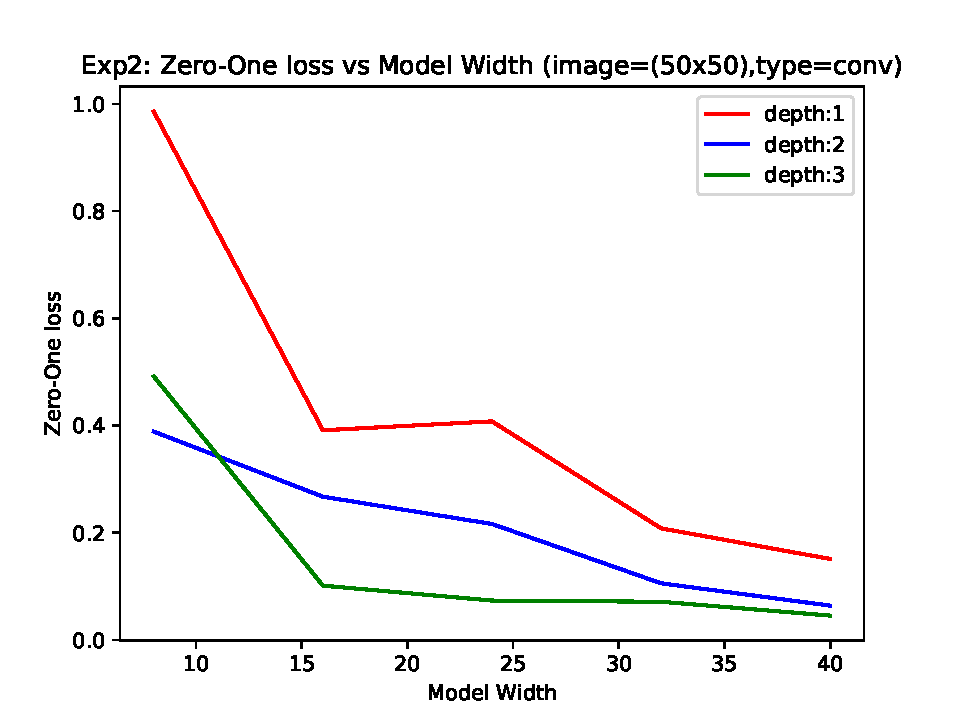
\includegraphics[width=\textwidth]{e2_50_conv_loss_width}
\caption{Experiment 2: zero-one loss vs ANN size}\label{fig:e2_50_loss_width}
\end{figure}

Results can be reproduced by following the steps highlighted in section\ref{sec:repro}.
